\documentclass[twoside,letterpaper,10pt]{report}
\usepackage[spanish,backgroundcolor=green,textsize=small]{todonotes}
\usepackage[top=3cm,bottom=3cm,left=3cm,right=3cm]{geometry} 
\usepackage[utf8x]{inputenc}
\usepackage[spanish]{babel}

\renewcommand{\familydefault}{\sfdefault} 
\usepackage{helvet}

\usepackage{amsmath}
\usepackage{amssymb}
\usepackage{times}
\usepackage{color}
\usepackage{graphicx}
\usepackage{framed}
\usepackage{wrapfig}
\usepackage{hyperref}
\usepackage{parskip}
\usepackage{float}
\usepackage[section]{placeins} 
%\usepackage[table]{xcolor}
%\usepackage{plain} % no se de que es
%\usepackage{a4wide} % para el ancho de pagina
%\usepackage{multirow} % tablas con multicolumna

\setlength{\parindent}{15pt}

\hypersetup{
colorlinks=true,
linkcolor=black,          % color of internal links (change box color with linkbordercolor)
citecolor=black,        % color of links to bibliography
filecolor=black,      % color of file links
urlcolor=black           % color of external links
}

\usepackage{listings}
\usepackage{courier}
\lstset{
basicstyle=\footnotesize\ttfamily, % Standardschrift
numbers=left,               % Ort der Zeilennummern
numberstyle=\tiny,          % Stil der Zeilennummern
%stepnumber=2,               % Abstand zwischen den Zeilennummern
numbersep=5pt,              % Abstand der Nummern zum Text
tabsize=2,                  % Groesse von Tabs
extendedchars=true,         %
breaklines=true,            % Zeilen werden Umgebrochen
keywordstyle=\color{red},
frame=b,         
%        keywordstyle=[1]\textbf,    % Stil der Keywords
%        keywordstyle=[2]\textbf,    %
%        keywordstyle=[3]\textbf,    %
%        keywordstyle=[4]\textbf,   \sqrt{\sqrt{}} %
stringstyle=\color{white}\ttfamily, % Farbe der String
showspaces=false,           % Leerzeichen anzeigen ?
showtabs=false,             % Tabs anzeigen ?
xleftmargin=17pt,
framexleftmargin=17pt,
framexrightmargin=5pt,
framexbottommargin=4pt,
%backgroundcolor=\color{lightgray},
showstringspaces=false      % Leerzeichen in Strings anzeigen ?        
}
\lstloadlanguages{% Check Dokumentation for further languages ...
%[Visual]Basic
%Pascal
%C
sh,
C++
%XML
%HTML
%Java
}

\title{
Carrera Solar de Derivadas y Aceleración\\
Propuesta de objeto de aprendizaje\\[0.5cm]
Libro de Producción}

\date{\today}

\author{
	Manuel Alejandro Gómez Rueda\\
	Sergio Andrés Monsalve Castañeda \\[2cm]
	Docentes\\[0.5cm]
	Alejandra Montoya\\
	Diego Montoya\\[1cm]
	Maestría en Ingeniería \\[1cm]
	%Universidad EAFIT\\[3cm]
	% Copyright \copyright \hspace{3pt}	\\
	
\includegraphics[width=0.25\textwidth]{aux/logo_eafit}
}


\begin{document}
\maketitle

\tableofcontents
\begin{abstract}
Este documento agrupa las entregas realizadas en la materia de Producción de Contenidos de Aprendizaje perteneciente a la Maestría en Ingeniería con especialización en Tecnologías de la Información y Comunicación para la Educación.
\end{abstract}

\chapter{Primera Entrega: Momento 1}

\section{¿Qué se va a hacer?}

\subsection{Contexto} % (fold)
\label{sub:contexto}

La presente propuesta de Objeto de Aprendizaje toma como punto de partida los enfoques y modelos educativos que en la actualidad se utilizan en la Universidad EAFIT para la enseñanza de temas que se enmarcan en las ciencias básicas (cálculo, física, estadística, entre otras) y que representan un reto para la Institución debido a las tasas importantes de pérdida de este tipo de asignaturas y a los vacíos que los estudiantes traen de niveles educativos inferiores.

Esta propuesta busca explorar herramientas tecnológicas y metodológicas que permitan a los estudiantes visualizar cómo los modelos matemáticos, y sus diferentes componentes, pueden tener una aplicación en el mundo real y son útiles para el desarrollo de algunas de las habilidades necesarias para un buen desempeño dentro de sus profesiones.

En primera instancia el objetivo es intervenir en el proceso educativo llevado a cabo en las materias de Calculo 1 y Física 1 que se dictan en las carreras de Ingeniería. 

\todo[inline,caption={TODO}]{Acá van las Estadísticas}
% subsection contexto (end)

\subsection{Cómo se imparte en la actualidad la estrategia de aprendizaje} % (fold)
\label{sub:c_mo_se_imparte_en_la_actualidad_la_estrategia_de_aprendizaje}

En la actualidad, las materias de ciencias básicas, sobre todo las que tienen que ver con cálculo, tienen una estrategia conductista enfocada en horas de asistencia a clases magistrales, trabajo independiente destinado a la realización de ejercicios y presentación de pruebas evaluativas.

El Objeto de aprendizaje que aquí se propone, buscará explorar estrategias como el aprendizaje por descubrimiento para mejorar el proceso de enseñanza y aprendizaje de esta área del conocimiento.

% subsection c_mo_se_imparte_en_la_actualidad_la_estrategia_de_aprendizaje (end)

\section{¿Quién es el destinatario?} % (fold)
\label{sec:_qui_n_es_el_destinatario_}

El público destinatario del objeto de aprendizaje de esta propuesta está conformado por estudiantes de los pregrados en Ingeniería Mecánica, Civil, de Sistemas, de Producción, de Procesos y Geología de la Escuela de Ingeniería de la Universidad EAFIT que cursan las asignaturas Cálculo 1 y Física 1 entre el primer el tercer semestre de sus carreras.

Para este segmento de población, encontrar formas en las que se apliquen las teorías de estas materias a través de historias relacionadas con temas cotidianos o con sus gustos, puede servir como aspecto motivador para incrementar su interés por los temas, ya que, al vivir en un mundo tan visual y mediatizado, suelen estar acostumbrados a tener mejor relación con lo que experimentan de primera mano.

Estos estudiantes, en su mayoría hombres colombianos, entre 18 y 22 años, centran su atención, de forma usual, en su círculo social y las actividades que les permiten placer y esparcimiento.

De esta forma, las discotecas, los bares, los restaurantes, las fincas, los lugares en los que pueden practicar sus hobbies (pistas, lagos, campos, canchas o gimnasios), son sitios que despiertan en buena medida sus intereses.

Otros aspectos que también llaman la atención de estos estudiantes son el fútbol (tanto nacional como europeo), los deportes extremos, los vehículos (bicicletas, motos y carros), la música de moda (tropical, urbana o electrónica), la ropa de moda, la tecnología (smartphones, juegos de video o equipos de cómputo) y los viajes. 

Este sector de población, que en su mayoría vive en sectores de estratos 4, 5 y 6 del área metropolitana de Medellín, estudia en la Universidad EAFIT con los recursos económicos que le brindan sus padres, con créditos estudiantiles o con becas, y reciben como parte de su formación enseñanzas con casos de éxito relacionados con el empresarismo que van de la mano, en algunas ocasiones, de las experiencias empresariales de sus propias familias.

Por esto, crear ideas nuevas o negocios nuevos, abordar los problemas desde enfoques diferentes, interesarse por aportar y asesorar proyectos, y depender de sus propias iniciativas, son actitudes comunes en ellos.

De otro lado, en su formación universitaria también encuentran retos relacionados con actividades comunicativas a idiomas diferentes al español (sobre todo inglés y, de forma reciente, francés, portugués y mandarín) y el trabajo en equipos multidisciplinarios.

Durante las clases usan cuadernos, computadores portátiles o tabletas para tomar notas y suelen formar grupos de trabajo para desarrollar talleres y preparar eventos evaluativos. 

Intervienen en clase para aportar de su experiencia o sus inquietudes, pero, si aún quedan con dudas después de una explicación, suelen no expresarlas. En general, guardan silencio cuando el profesor pregunta ¿tienen alguna duda?

Su relación con el profesor, por fuera de la clase, se da en los momentos en los que requieren asesoría o no están de acuerdo con las calificaciones. Estos encuentros suceden en diferentes partes del campus, en la oficina del docente, a través de la plataforma EAFIT Interactiva o por correo electrónico. 

Son personas que consumen pocos medios noticiosos tradicionales, leen poco en medios físicos, usan mucho los servicios de redes sociales digitales públicas y son apáticos en temas políticos.

Son personas que permanecen varias horas diarias en internet, a través de computadores o dispositivos móviles, relacionándose con sus pares, consultando y compartiendo contenido sobre sus intereses y realizando actividades que ayuden a su formación profesional (viendo videos, buscando información, presentando exámenes).

\newpage

% section _qui_n_es_el_destinatario_ (end)

\subsection{Arquetipos} % (fold)
\label{sub:arquetipos}

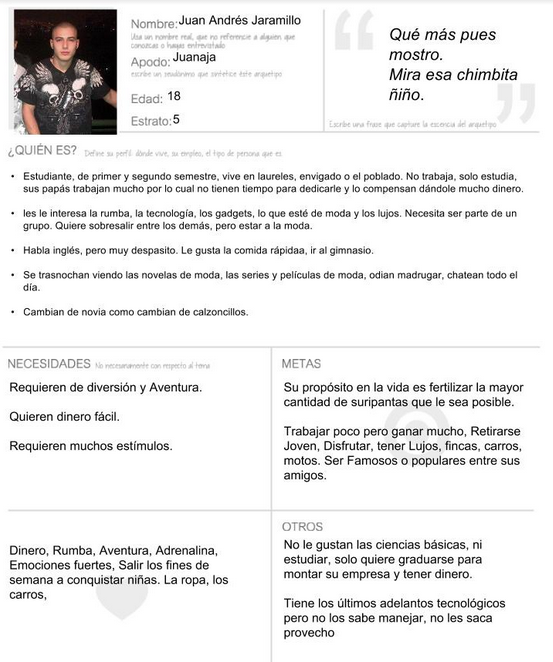
\includegraphics[width=1\textwidth]{aux/arquetipo1}

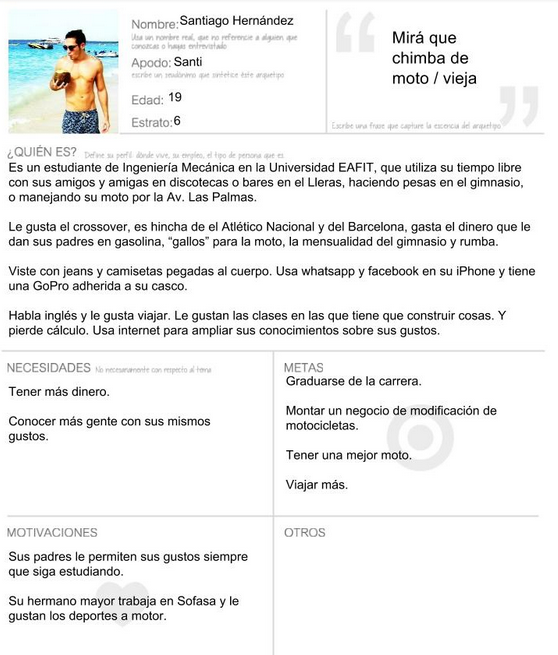
\includegraphics[width=1\textwidth]{aux/arquetipo2}

% subsection arquetipos (end)

\section{¿En qué consiste y por qué es pertinente el objeto de aprendizaje?} % (fold)
\label{sec:_en_qu_consiste_y_por_qu_es_pertinente_el_objeto_de_aprendizaje_}

\subsection{Conceptos y temas de interés} % (fold)
\label{sub:conceptos_y_temas_de_inter_s}

\todo[inline,caption={TODO}]{compelentar}

\subsection{Qué contiene y por qué un OA soluciona el problema} % (fold)
\label{sub:qu_contiene_y_por_qu_un_oa_soluciona_el_problema}

El objeto de aprendizaje que se propone en este trabajo es un ambiente web en el que el estudiante encuentra la explicación de un tema relacionado con matemáticas y física a través de recursos multimedia que lo guían por explicaciones teóricas, demostraciones de la teoría y un ambiente de simulación en el que el estudiante puede manipular un modelo matemático y descubrir su aplicación.

Esta serie de recursos tienen como eje transversal una historia en la que el estudiante tiene el reto de intervenir par ayudar a solucionar un problema.

Con esta estrategia se pretende que el alumno pueda vislumbrar, a través de un ejercicio simulado, que aprender teorías matemáticas es útil para resolver problemas del mundo real y a los que podría enfrentarse en un futuro como profesional.

Utilizar historias como la construcción del puente que une el campus de EAFIT con el lote de Los Guayabos, la desviación del río Cauca para la construcción de Hidroituango, construir una de las nuevas autopistas del Departamento de Antioquia, o hacer una carrera de cuarto de milla en la Avenida Regional y otras de las que puedan tener referencias cercanas, son un recurso que puede despertar el interés por aprender nuevas teorías desde sus posibles aplicaciones.  

\todo[inline,caption={TODO}]{Complementar}



% subsection qu_contiene_y_por_qu_un_oa_soluciona_el_problema (end)

% subsection conceptos_y_temas_de_inter_s (end)
% section _en_qu_consiste_y_por_qu_es_pertinente_el_objeto_de_aprendizaje_ (end)

\section{Objetivos del objeto de aprendizaje} % (fold)
\label{sec:objetivos_del_objeto_de_aprendizaje}

\subsection{Objetivo General} % (fold)
\label{sub:objetivo_general}

Orientar al estudiante en el aprendizaje de conceptos y teorías de las asignaturas Cálculo 1 y Física 1 a partir de la exploración de explicaciones demostrativas multimedia y la simulación de problemas de ingeniería que guarden relación con situaciones que puedan resultar atractivas o cotidianas para los estudiantes.

% subsection objetivo_general (end)

\subsection{ Objetivos Específicos} % (fold)
\label{sub:_objetivos_espec_ficos}

\begin{itemize}
	\item Facilitar la comprensión de conceptos como función, derivada y relación de cambio, propios del Cálculo, a partir de explicaciones teóricas y demostraciones de sus aplicación en fenómenos de la vida real.

	\item Explicar los conceptos de movimiento, velocidad, distancia, tiempo y aceleración, propios de la cinemática en Física, valiéndose del análisis del movimiento de objetos comunes para el estudiante y de los modelos matemáticos que allí tengan cabida.

	\item Relacionar los conceptos de ambas áreas del conocimiento, mediante un ambiente de simulación que puede ser alterado por el estudiante, con el fin de demostrar la convergencia de los modelos matemáticos y los fenómenos físicos en una misma situación determinada.

	\item Invitar al estudiante a alterar las partes del fenómeno, en un ambiente simulado, para que logre comprender las relaciones de cambio en un modelo matemático y los efectos físicos que se pueden producir.

	\item Propiciar el aprendizaje de estos conceptos con contenidos multimedia que puedan simular el movimiento de los objetos y que se puedan relacionar con los gustos que puedan tener la mayoría de los estudiantes.

\end{itemize}

% subsection _objetivos_espec_ficos (end)

\subsection{Competencias que el objeto de aprendizaje desarrollará en los estudiantes } % (fold)

\todo[inline,caption={TODO}]{Complementar}

% subsection competencias_que_el_objeto_de_aprendizaje_desarrollar_en_los_estudiantes_ (end)
% section objetivos_del_objeto_de_aprendizaje (end)


\chapter{Segunda Entrega: Momento 2}

\section{Tipología textual}

En el objeto de aprendizaje de esta propuesta se usarán textos informativos e interactivos enmarcados en un texto narrativo transversal.

\subsection{Texto narrativo} % (fold)
\label{sub:texto_narrativo}

El contexto que rodea este objeto de aprendizaje comienza en el aula de clase, donde un docente de Cálculo 1 o Física 1, presenta a sus alumno este recurso de aprendizaje y anuncia los beneficios que pueden obtener al usarlo.

La Carrera Solar de Derivadas y Aceleración es un certamen de carreras de cuarto de milla de carros solares que se desarrolla a lo largo del sector de la Avenida Regional adyacente al Campus Medellín de la Universidad EAFIT.

El reto para los estudiantes de los diferentes pregrados en ingeniería que participen es proponer la mejor manera de hacer que su carro recorra esa distancia y pueda ganar la carrera.

Para lograr esta tarea, se presentan algunas ayudas (simulaciones de movimiento y explicaciones de fenómenos físicos y matemáticos) que pueden guiar hacia la respuesta.

Una vez los estudiantes de un curso conocen y recorren esta experiencia, envían su propuesta al profesor, quien anuncia al ganador de la carrera y el premio que se le otorga.

Con este texto narrativo se pretende involucrar la actividad en clase con la actividad en línea. 

Se usa el concepto de carrera con el fin de generar interés competitivo en los estudiantes que, además, pueda motivar el aprendizaje de los diferentes temas relacionados para proponer un mejor resultado.

Además, se usan referencias cercanas a estudiantes de EAFIT, como carros solares, la Avenida Regional y el campus de la Universidad con la meta de que el alumno comprenda que la situación planteada se puede presentar en la vida real y que lo que aprende tiene aplicaciones prácticas.

% subsection texto_narrativo (end)

\subsection{Texto explicativo} % (fold)
\label{sub:texto_explicativo}

Estos textos son parte de las ayudas que tendrán los estudiantes para participar en la carrera.

Se usan formatos como video y texto escritos de acompañamiento que expliquen los conceptos que se deben usar para la solución del problema.

Los videos que se usan explican el tema por fuera del tablero. Usan un lenguaje más cercano y ayudas visuales que facilitan el entendimiento de los fenómenos físicos implicados en el movimiento acelerado y las herramientas matemáticas (ecuaciones y derivadas) que permiten comprenderlos.

Este objeto de aprendizaje no exige una lectura lineal del contenido, por lo que la comprensión de los temas en la que derivaría la lectura de este tipo de texto puede darse, incluso, de manera posterior a la solución propuesta por el estudiante.

% subsection texto_explicativo (end)

\subsection{Texto interactivo} % (fold)
\label{sub:texto_interactivo}

El objetivo que se persigue con este tipo de texto es que el alumno entienda la relación entre las variables de un modelo matemático y los efectos del cambio en estas sobre un fenómeno físico.

Además, la manipulación del modelo afectará la representación visual del mismo, lo que permitirá al estudiante experimentar con el análisis de gráficos.

De esta manera, el participante puede obtener información adecuada para pensar en una propuesta de solución al problema planteado.

% subsection texto_interactivo (end)

\section{Tipología del objeto de aprendizaje} % (fold)
\label{sec:tipolog_a_del_objeto_de_aprendizaje}

Debido a que en esta propuesta se plantea el uso de diferentes tipos de texto explicativo y a que el texto interactivo se accede a través de un servicio en línea, se determina que un ambiente web es el mejor medio para ejecutar esta experiencia de aprendizaje.

Esto permitirá que el estudiante se pueda tomar el tiempo necesario para recorrerla usando cualquier computador con acceso a internet (el ambiente de simulación de esta experiencia requerirá que el usuario descargue e instale un plug-in que permite su funcionamiento).

Este entorno web se alojará dentro del Portal Web de la Universidad EAFIT con el fin de permitir su acceso y de ayudar al contexto cercano que pretende el objeto de aprendizaje.
 
A partir de esta decisión también se determina que la presente propuesta puede tener aplicación para temas diferentes a derivadas y movimiento acelerado, por lo que La Carrera Solar de Derivadas y Aceleración constituye un capítulo de una serie de objetos de aprendizaje. 

Esta situación lleva a pensar en un servicio de objetos de aprendizaje, que se denominó Escuela Abierta, que tendría una sección dedicada a la física y las matemáticas básicas denominada Problemas de Garaje en la que estaría presente la presente experiencia (Ver Figura ~\ref{esbozos}). 

\begin{figure}[h!]
\label{esbozos}
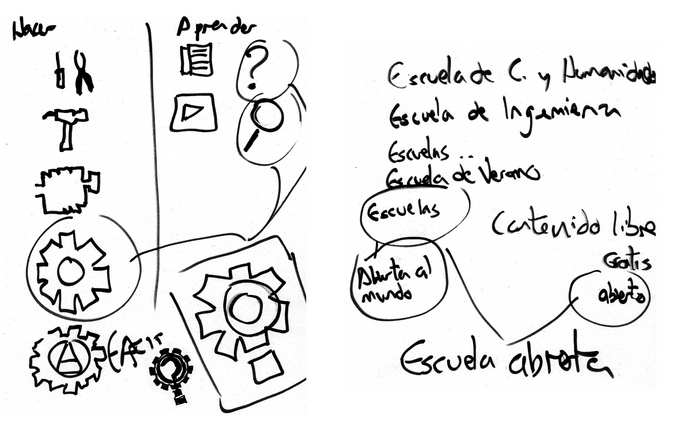
\includegraphics[width=1\textwidth]{aux/esbozos}
\caption{\textbf{Esbozos de la identidad gráfica de Escuela Abierta.}}
\end{figure}


% section tipolog_a_del_objeto_de_aprendizaje (end)

\section{Planteamiento estético} % (fold)
\label{sec:planteamiento_est_tico}

Como en este objeto de aprendizaje no se obliga una lectura secuencial, el diseño de la experiencia web incluirá una navegación que le permita opciones, antes que obligaciones, al estudiante.

En consecuencia, se busca un diseño en el que la mayoría de la información se despliegue en una pantalla sin necesidad de que el participante use el scroll y con un menú siempre visible (ver Figura: ~\ref{sketches}).

\begin{figure}[h!]
\label{sketches}
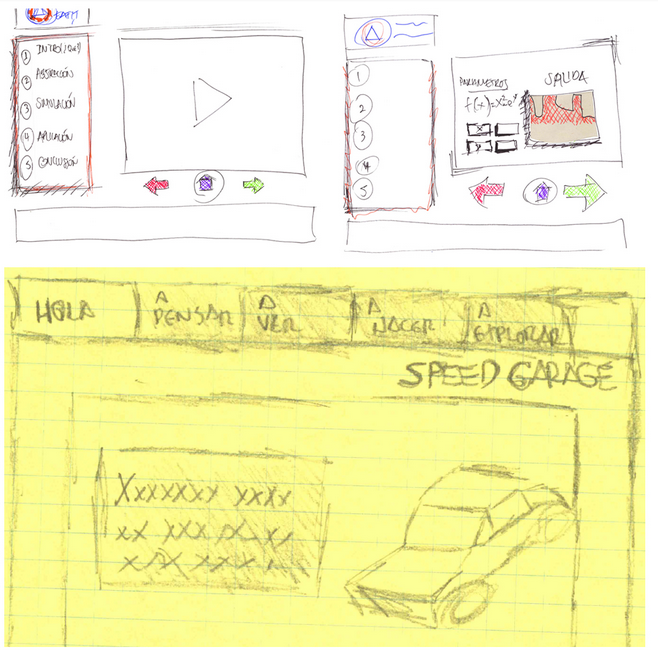
\includegraphics[width=1\textwidth]{aux/sketches}
\caption{\textbf{Sketches de dos propuestas de diseño del objeto de aprendizaje}}
\end{figure}


A partir de los primeros esbozos comenzó el diseño de la información, que en un primer momento consistió en definir los tipos de contenido que estarían presentes y luego en establecer una distribución que permitiera al estudiante tomar el camino que más desee.

Así, los contenidos se dividieron en secciones que tuvieran denominaciones destacadas o que llamaran a la acción: ¡Hola!, ups… un problema, una solución, tu solución, explorar más.

Esta serie de acciones permiten plantear una propuesta final mediante wireframes (ver Figura ~\ref{sketches}).

\begin{figure}[h!]
\label{wireframes}
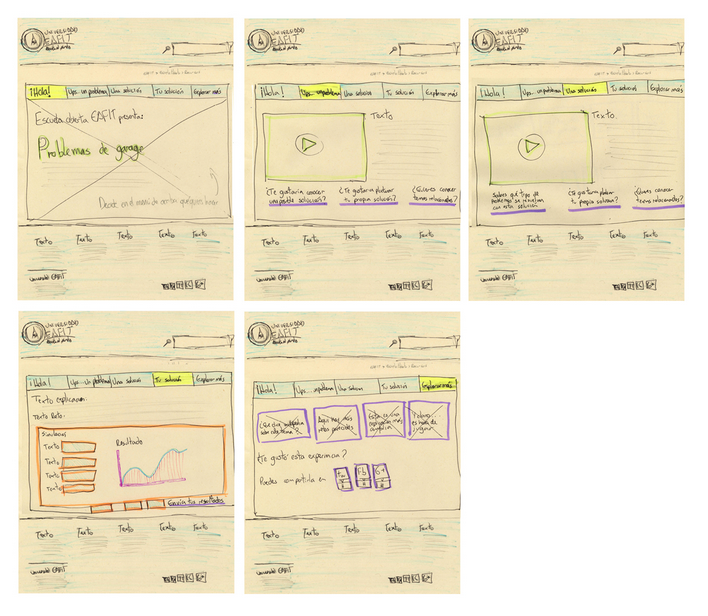
\includegraphics[width=1\textwidth]{aux/wireframes}
\caption{\textbf{Wireframes de la propuesta final de diseño enmarcados en el Portal Web de EAFIT.}}
\end{figure}


Con la propuesta de diseño clara, es tiempo de definir detalles que aportarán elementos comunicativos clave para el entorno de aprendizaje que se quiere diseñar.

Para esto, la descripción del público y el texto narrativo del objeto de aprendizaje evocan conceptos como carrera, actividad, juventud, tecnología, ecología, sol, movimiento, energía y luz, que deben estar representados en los colores y la tipografía que se utilice.

En el caso del color, también es pertinente tener en cuenta que la experiencia web está diseñada para estudiantes de la Universidad EAFIT y que, además, estará desplegada dentro de su Portal Web, lo que hace necesario asociar la estética del objeto de aprendizaje con la identidad de la Institución.

Así, entonces, se define una paleta de colores (ver Figura: ~\ref{paleta}) que incluye verde (ecología, energía), azul (tecnología, EAFIT), blanco (actividad, iluminación), y gris (por el contraste con el fondo se usará para los textos).
\begin{figure}[h!]
\label{paleta}
\centering
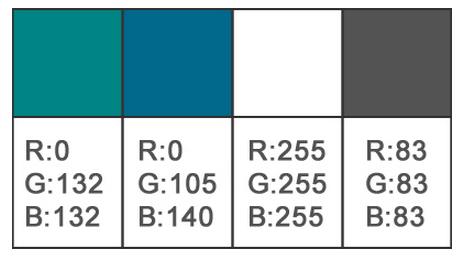
\includegraphics[width=0.5\textwidth]{aux/paletaColores}\caption{\textbf{Paleta de colores que se usará en el objeto de aprendizaje.}}
\end{figure}

En concordancia con el color, la tipografía debe reflejar tecnología, modernidad y ser adecuada para la lectura en pantalla. En consecuencia se utilizarán fuentes sin serifas y de trazos delgados (en el levantamiento digital de los wireframes se utilizó la familia Zurich, pero en el objeto final se utilizará la familia Helvética).

A estos aspectos se une la diagramación de la información.

Este objeto de aprendizaje constará de cinco secciones con diferentes tipos de diagramación según las necesidades informativas y didácticas.

Las secciones de bienvenida y de simulación tendrán diagramación de una columna, porque allí se darán instrucciones importantes y se realizarán las actividades que más atención requieren, por lo que tener información en el centro de la pantalla es fundamental.

Las secciones de planteamiento de problema y explicación del tema tendrán diagramación combinada de una y dos columnas, con el fin de tener información complementaria y varios formatos de texto.

La sección de referencias tendrá diagramación combinada de una y tres columnas, debido a que se usarán textos cortos y se pretende publicar muchos recursos externos.

En suma, estos elementos permiten hacer un levantamiento digital de los wireframes de la propuesta final y tener una idea general de la propuesta estética del objeto de aprendizaje (Ver Figura ~\ref{prupuesta}).


\begin{figure}[h!]
\label{propuesta}
\centering
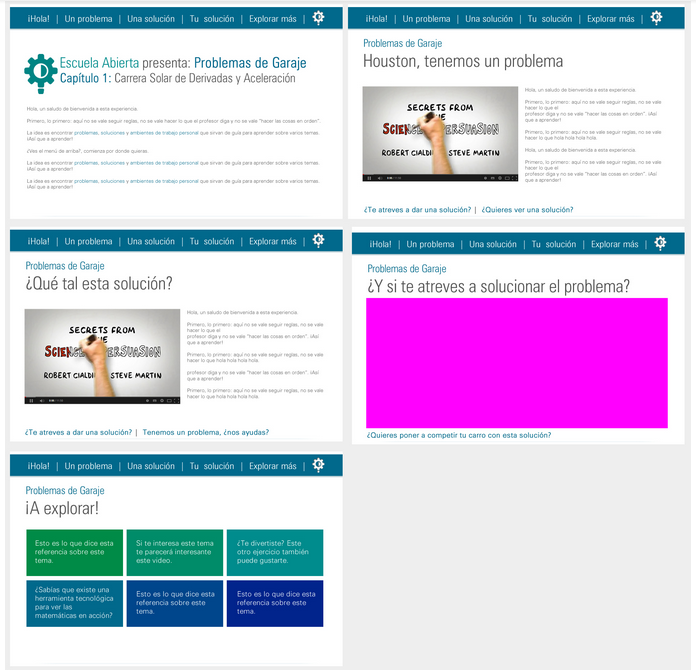
\includegraphics[width=1\textwidth]{aux/propuestaEstetica}
\caption{\textbf{Propuesta estética del objeto de aprendizaje.}}
\end{figure}

acá algo para citar del libro ese de la margarita\cite{5seg}


\bibliographystyle{ieeetr}
\bibliography{Referencias.bib}

\newpage

\appendix
\chapter{Repositorio}

La versión actualizada de este documento se puede encontrar aquí:\\
 \url{https://raw.githubusercontent.com/smonsalve/OA/master/OA.pdf}

Los siguientes documentos son relevantes para este trabajo, en el link adjunto podrán descargar una copia de los mismos:

\begin{itemize}

	\item 	\href{https://github.com/smonsalve/OA/blob/master/Apendices/1%20CB0240pdf.pdf?raw=true}
	{Programa de la Universidad EAFIT para Calculo 1.}

	\item 	\href{https://github.com/smonsalve/OA/blob/master/Apendices/1%20CB0236pdf.pdf?raw=true}
	{Programa de la Universidad EAFIT para Física 1.}

	\item \href{https://github.com/smonsalve/OA/blob/master/Apendices/EstadisticasDepuradas.xlsx?raw=true}
	{Estadísticas materias relacionadas con ciencias Básicas, discriminadas por ingenierías (Civil, Mecánica, Procesos, Producción Sistemas y Geología)}

	\item \href{https://github.com/smonsalve/OA/blob/master/Apendices/Calculo1.xlsx?raw=true}
	{Estadísticas para Calculo 1 discriminadas por años.}

	\item \href{https://github.com/smonsalve/OA/blob/master/Apendices/Fisica1.xlsx?raw=true}
	{Estadísticas para Física 1 discriminadas por años.}

\end{itemize}

\end{document}
